  \documentclass[14pt, oneside]{book}
    \usepackage[margin=1in]{geometry} 
    \usepackage[brazilian]{babel}
    \usepackage{graphicx}
    \usepackage[utf8]{inputenc}
    \usepackage[T1]{fontenc}
    \usepackage{amsmath,amsthm,amssymb,amsfonts}
    \usepackage{enumitem}
    \usepackage{multicol}
    \usepackage{subfig}
    \usepackage{mathtools}
    \usepackage{titlesec}
    \usepackage{listings}
    \usepackage{float}
    \titleformat{\chapter}[hang]{\bf\huge}{\thechapter}{2pc}{}
    \DeclarePairedDelimiter{\ceil}{\lceil}{\rceil}
    \lstset{language=Python}  
    \usepackage{pythonhighlight}
     
    \newcommand{\N}{\mathbb{N}}
    \newcommand{\Z}{\mathbb{Z}}
    \newcommand\tab[1][1cm]{\hspace*{#1}}
    \renewcommand{\qedsymbol}{$\blacksquare$}
     
    
\theoremstyle{definition}
    \newtheorem{problem}{Problema}
    \newtheorem{dica}{Dica}
    \newtheorem{gabarito}{Gabarito}
    \newtheorem{defn}{Definição}
    \newtheorem{teorema}{Teorema}
    
    
\begin{document}
    \pagenumbering{gobble}

    \begin{titlepage}
        \centering 
        
\includegraphics[scale = 0.8]{ufpe.png} \\
        \Large{\textbf{UNIVERSIDADE FEDERAL DE PERNAMBUCO}}\\
        \large{Departamento de Eletrônica e Sistemas}
        \vspace*{\stretch{2.0}}
   
        \Huge\textbf{MEDIDAS ELETROMAGNÉTICAS}\\
        \Large\textbf{SISTEMA DE MEDIÇÃO INDIRETA DE TEMPERATURA}
   
        \vspace*{\stretch{2.0}}
        \vfill
        \Large{Arthur Santos Pimentel} \\
        \Large{Matheus Sobreira Farias} \\
        \Large{Victor Gouveia Menezes Lyra}
        \\~\\
        \Large{Abril 2018}
    \end{titlepage}

    
    \mainmatter
        \chapter{Apresentação}
            \tab A temperatura é uma das variáveis mais importantes na natureza, e não seria diferente na engenharia. O controle de seu nível mostra-se bastante relevante nas indústrias, onde, por exemplo, em uma reação química é necessário que a temperatura mantenha-se constante ao longo de todo o processo. Dessa forma, é possível citar diversos modos de realizar medições precisas de seu valor, no presente trabalho foi usado uma medição indireta, visto que a temperatura foi obtida através de um sensor que acusa a diferença de potencial tal qual se relaciona com a temperatura proporcionalmente. \\
            \tab O trabalho, portanto, tem como objetivo a confecção de uma placa de circuito impresso que medirá a temperatura de um mensurando dentro das normas da metrologia científica, se preocupando com as incertezas dos instrumentos utilizados, bem como a rede elétrica do local e o ganho fornecido pelo circuito.
                
    \tableofcontents
    
        \chapter{Introdução}
            \tab Ao analisar o funcionamento de um circuito, um equipamento, um instrumento ou até mesmo um componente eletrônico, é necessário efetuar medidas e utilizar uma metodologia adequada para cada tipo de avaliação, tendo sempre o cuidado de expressar as medidas com clareza, precisão adequada e com suas unidades convenientemente padronizadas. \\
            \tab Para o desenvolvimento do sistema de medição, foi utilizado o sensor de temperatura LM$35$, que, ao receber a alimentação necessária entre seus terminais ($4/30$ V), gera uma tensão de saída que, ao receber o ganho de $10$ pelo amplificador operacional LM$741$ na configuração de inversor, com dois resistores de valor nominal $10$ k$\Omega$ e $100$ k$\Omega$, será medida com a ajuda de um voltímetro. \\
            \tab No entanto, como se é estudado na disciplina de Medidas Eletromagnéticas, tais medições não são exatas, cada etapa possui sua devida incerteza, e cabe ao projetista avaliar, com base no padrão estabelecido pela metrologia científica, se ao fim de cada etapa o resultado é o desejado.
              
        \chapter{Objetivos}
            \tab O objetivo principal é confeccionar uma placa de circuito impresso, projetada no software \textit{Proteus}, que possa, de forma indireta, medir a temperatura de um mensurando, através do uso do sensor LM$35$, e, durante esse processo, observar na prática toda a teoria estudada na disciplina de Medidas Eletromagnéticas, que está relacionada com o cuidado necessário ao trabalhar com as incertezas e com os padrões de medição para então avaliar se o produto final atende a tais normas.
            
         \chapter{Metodologia}
            \section{Projeto da Placa}
                \tab Antes de iniciar a confecção da placa propriamente dita, é necessário realizar o projeto, para isso, foi utilizado o software \textit{Proteus}. Primeiramente foi feito o esquema do circuito na plataforma \textit{ISIS} para checar se o resultado simulado é o que se espera (Figuras \ref{inicio} e \ref{top} abaixo). \\
                %figura 1 - esquema inicial do isis
                \begin{figure}[H]
                    \centering
                    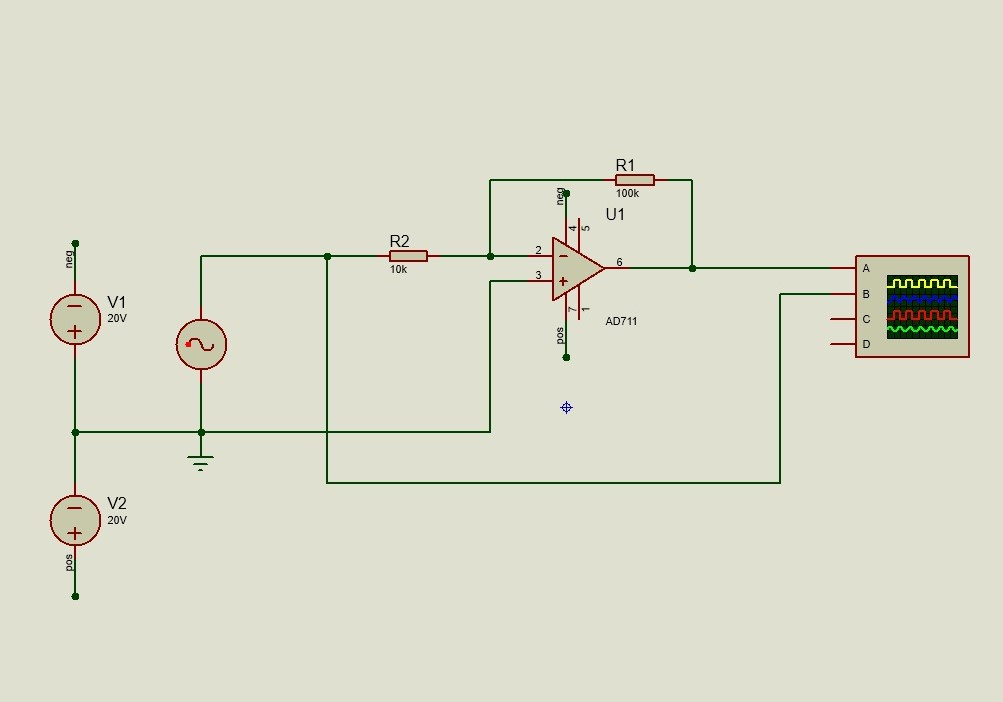
\includegraphics[scale= 0.32]{Simulacao_circuito(osciloscopio).jpeg}
                    \caption{Esquema Inicial do $ISIS$}
                    \label{inicio}
                \end{figure}
                %figura 2 - saida do osciloscopio
                \begin{figure}[H]
                    \centering
                    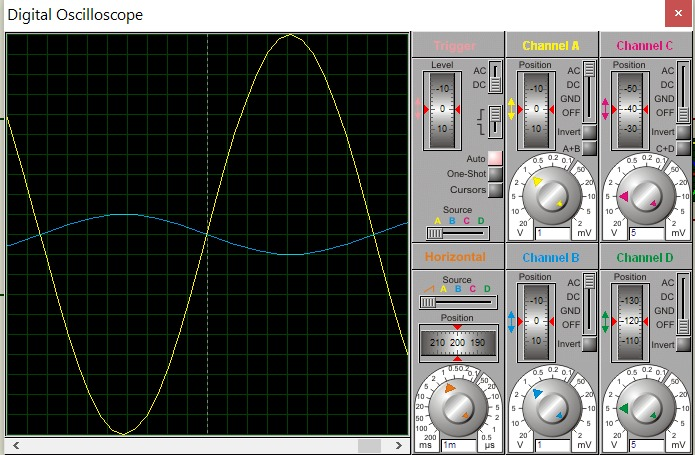
\includegraphics[scale= 0.35]{Osciloscopio.jpeg}
                    \caption{Saida do Osciloscópio}
                    \label{top}
                \end{figure}
                \tab Após a simulação, foram colocados os conectores no esquema do circuito e depois foi feito o seu layout na plataforma \textit{ARES} tendo os cuidados fundamentais de espaçamento de trilha e ilhas de solda, para que não ocorra nenhum curto no circuito (Figuras \ref{novo} e \ref{dale}). \\
                %figura 3 - esquema do isis com os conectores%
                \begin{figure}[H]
                    \centering
                    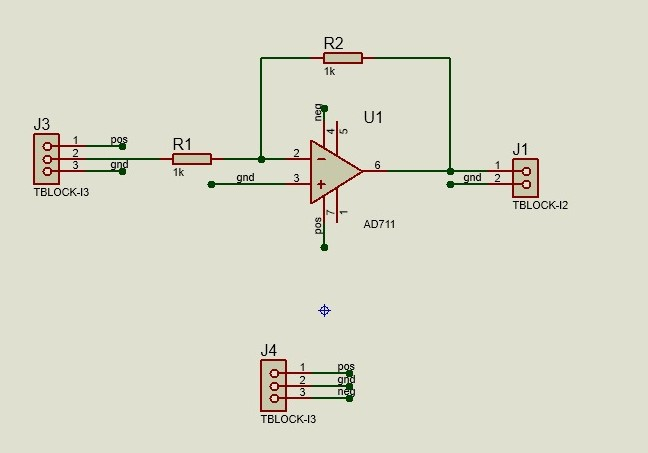
\includegraphics[scale= 0.46]{circuito(tblock).jpeg}
                    \caption{Esquema do $ISIS$ com Conectores}
                    \label{novo}
                \end{figure}
                %figura 4- esquema no ares%
                \begin{figure}[H]
                    \centering
                    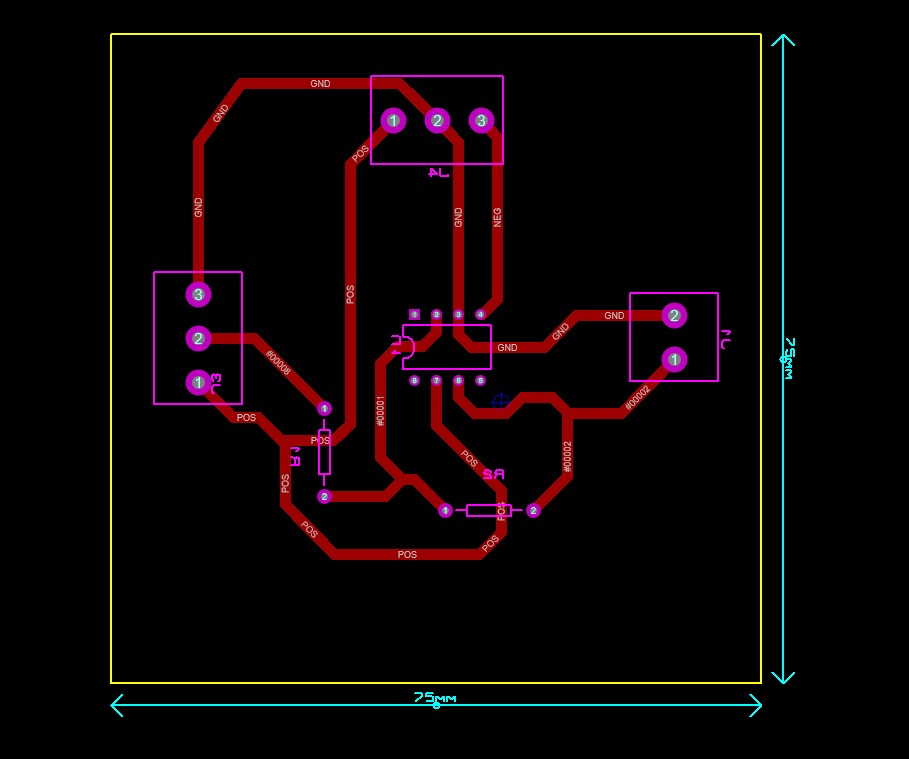
\includegraphics[scale= 0.25]{circuito(proteus).jpeg}
                    \caption{Esquema no $ARES$}
                    \label{dale}
                \end{figure} \\
                \tab Passado as simulações e ajustes computacionais, a placa foi impressa em papel fotográfico e com a prensa foi gravada em uma placa de fenolite após uma limpeza bastante cuidadosa para evitar marcas de oleosidade ou resíduos em sua superfície. \\
                %figura 5 - layout da placa impresso%
                \begin{figure}[H]
                    \centering
                    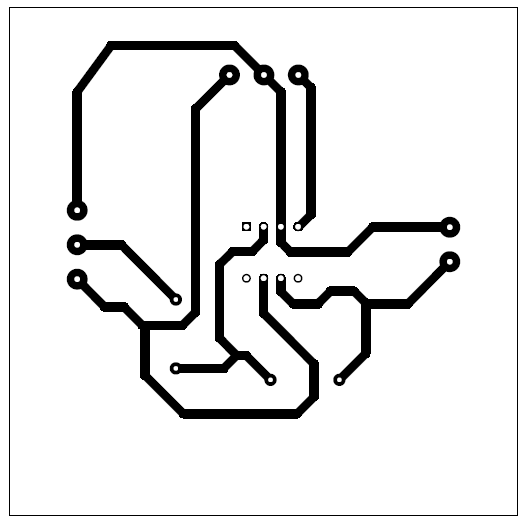
\includegraphics[scale= 0.8]{Layout_Placa}
                    \caption{Layout da Placa}
                    \label{fig:my_label5}
                \end{figure}
                \tab Com o circuito devidamente gravado na placa de fenolite, esta foi imersa em uma solução de percloreto de ferro FeCl$_3$ para que fosse corroída. Depois de algumas horas corroendo, a placa foi retirada, lavada e perfurada, para que finalmente fosse realizada a soldagem dos elementos eletrônicos. Por fim, foi feito o teste de continuidade nas trilhas com um multímetro.
            
            \section{Avaliação dos Resistores}
                \tab Nesta etapa do projeto, foi utilizado dois lotes de $15$ resistores para avaliação, sendo um deles com valor nominal de $10$ k$\Omega$ e o outro com valor nominal de $100$ k$\Omega$, sendo os valores de resistência medidos pelo multímetro digital \textit{ET-2042C}. Através do conhecimento de técnicas de análise de circuitos elétricos, é fácil perceber que o ganho $G$ do circuito amplificador inversor mostrado na Figura \ref{ampop} é dado pela equação \ref{ganho} abaixo:
                \begin{equation}
                    G = \frac{R_2}{R_1}
                    \label{ganho}
                \end{equation}
                \begin{figure}[H]
                    \centering
                    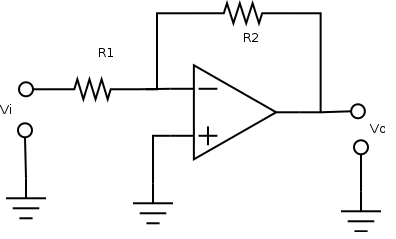
\includegraphics[scale = 0.8]{figura6.png}
                    \caption{Amplificador Operacional Inversor}
                    \label{ampop}
                \end{figure}
                \tab Dentre os $20$ resistores, foram escolhidos os que mais se aproximam, nominalmente, de $10$ k$\Omega$ e $100$ k$\Omega$.
            
            \section{Avaliação da Rede Elétrica}
                \tab Para realizar a avaliação da rede elétrica do local foram feitas $10$ medições diferentes utilizando $3$ multímetros distintos simultaneamente em paralelo, sendo as medidas espaçadas de pelo menos $30$ minutos.
                
            \section{Avaliação dos Instrumentos de Medição}
                \tab Para realizar a avaliação dos instrumentos de medição utilizados no projeto, foram medidos os valores médios quadráticos das tensões (valores \textit{RMS}) nos formatos de onda senoidal, quadrático e triangular, cada uma delas em três amplitudes diferentes: $1$, $1,5$ e $2$ V e em três frequências diferentes: $60$ Hz, $600$ Hz e $6$ kHz e os três multímetros usados foram: Multímetro Digital \textit{ ET-2042C}, Multímetro Analógico \texit{MXT YX-360TRN} e Multímetro \textit{True RMS Meterman 38XR} com o sinal de saída sempre monitorado pelo osciloscópio.
                
            \section{Avaliação do Amplificador Operacional}
                \tab O circuito com amplificador tem o objetivo de retornar a tensão de saída sendo $10$ vezes maior do que a tensão de entrada, essa avaliação busca reconhecer se o amplificador utilizado LM$741$ realmente atendeu à necessidade. Para isso, o amplificador foi alimentado com $+15$ V e $-15$ V e a entrada com $1$ V, para que fosse esperado uma saída de $10$ V.
                
            \section{Avaliação do LM$35$ e Sistema}
                \tab Para realizar as medições primeiramente foi estabelecido quais mensurando iam ser analisados, o mais simples e primeiro foi a própria temperatura ambiente do Laboratório Didático de Eletrônica. \\
                \tab Posteriormente pensou-se em medir um copo com água gelada, porém por conta da dificuldade de medição e o cuidado extremo que se deveria ter para que não danificasse a placa, preferiu-se descartar essa ideia. Só entao foi decidido usar o próprio ferro de solda como mensurando. \\
                \tab Foi posicionado o LM$35$ e a ponteira do True RMS o mais próximo possível da base (para que não fosse medido a parte mais quente do ferro) e, com o ferro ligado na tomada, foi anotado duas temperaturas com uma boa distância.
                
                
        \chapter{Desenvolvimento}
        
            \section{Avaliação dos Resistores}
            
               
                							


            % ######## init table ########
                \begin{table}[h]
                    \centering
                    \label{resistores}
                    % distancia entre a linha e o texto
                    {\renewcommand\arraystretch{1.25}
                    \caption{Valores das resistências}
                    \begin{tabular}{ l l l l }
                        \cline{1-1}\cline{2-2}\cline{3-3}\cline{4-4}  
                            \multicolumn{1}{|p{3.033cm}|}{$R_1$ (k$\Omega$) \centering } &
                            \multicolumn{1}{p{2.267cm}|}{Erro (\%) \centering } &
                            \multicolumn{1}{p{4.217cm}|}{$R_2$ (k$\Omega$)\centering } &
                            \multicolumn{1}{p{4.217cm}|}{Erro (\%) \centering }
                  \\  
                        \cline{1-1}\cline{2-2}\cline{3-3}\cline{4-4}  
                            \multicolumn{1}{|p{3.033cm}|}{9,83 \centering } &
                            \multicolumn{1}{p{2.267cm}|}{1,7 \centering } &
                            \multicolumn{1}{p{4.217cm}|}{97,8 \centering } &
                            \multicolumn{1}{p{4.217cm}|}{2,2 \centering }
                  \\  
                        \cline{1-1}\cline{2-2}\cline{3-3}\cline{4-4}  
                            \multicolumn{1}{|p{3.033cm}|}{9,87 \centering } &
                            \multicolumn{1}{p{2.267cm}|}{1,3 \centering } &
                            \multicolumn{1}{p{4.217cm}|}{97,5 \centering } &
                            \multicolumn{1}{p{4.217cm}|}{2,5 \centering }
                  \\  
                        \cline{1-1}\cline{2-2}\cline{3-3}\cline{4-4}  
                            \multicolumn{1}{|p{3.033cm}|}{9,86 \centering } &
                            \multicolumn{1}{p{2.267cm}|}{1,4 \centering } &
                            \multicolumn{1}{p{4.217cm}|}{98,0 \centering } &
                            \multicolumn{1}{p{4.217cm}|}{2,0 \centering }
                  \\  
                        \cline{1-1}\cline{2-2}\cline{3-3}\cline{4-4}  
                            \multicolumn{1}{|p{3.033cm}|}{9,87 \centering } &
                            \multicolumn{1}{p{2.267cm}|}{1,3 \centering } &
                            \multicolumn{1}{p{4.217cm}|}{97,6 \centering } &
                            \multicolumn{1}{p{4.217cm}|}{2,4 \centering }
                          \\  
                        \cline{1-1}\cline{2-2}\cline{3-3}\cline{4-4}  
                            \multicolumn{1}{|p{3.033cm}|}{9,87 \centering } &
                            \multicolumn{1}{p{2.267cm}|}{1,3 \centering } &
                            \multicolumn{1}{p{4.217cm}|}{99,1 \centering } &
                            \multicolumn{1}{p{4.217cm}|}{0,9 \centering }
                          \\  
                        \cline{1-1}\cline{2-2}\cline{3-3}\cline{4-4}  
                            \multicolumn{1}{|p{3.033cm}|}{9,84 \centering } &
                            \multicolumn{1}{p{2.267cm}|}{1,6 \centering } &
                            \multicolumn{1}{p{4.217cm}|}{98,0 \centering } &
                            \multicolumn{1}{p{4.217cm}|}{2,0 \centering }
                          \\  
                        \cline{1-1}\cline{2-2}\cline{3-3}\cline{4-4}  
                            \multicolumn{1}{|p{3.033cm}|}{9,86 \centering } &
                            \multicolumn{1}{p{2.267cm}|}{1,4 \centering } &
                            \multicolumn{1}{p{4.217cm}|}{98,0 \centering } &
                            \multicolumn{1}{p{4.217cm}|}{2,0 \centering }
                          \\  
                        \cline{1-1}\cline{2-2}\cline{3-3}\cline{4-4}  
                            \multicolumn{1}{|p{3.033cm}|}{9,79 \centering } &
                            \multicolumn{1}{p{2.267cm}|}{2,1 \centering } &
                            \multicolumn{1}{p{4.217cm}|}{99,0 \centering } &
                            \multicolumn{1}{p{4.217cm}|}{1,0 \centering }
                          \\  
                        \cline{1-1}\cline{2-2}\cline{3-3}\cline{4-4}  
                            \multicolumn{1}{|p{3.033cm}|}{9,87 \centering } &
                            \multicolumn{1}{p{2.267cm}|}{1,3 \centering } &
                            \multicolumn{1}{p{4.217cm}|}{98,2 \centering } &
                            \multicolumn{1}{p{4.217cm}|}{1,8 \centering }
                          \\  
                        \cline{1-1}\cline{2-2}\cline{3-3}\cline{4-4}  
                            \multicolumn{1}{|p{3.033cm}|}{9,80 \centering } &
                            \multicolumn{1}{p{2.267cm}|}{2,0 \centering } &
                            \multicolumn{1}{p{4.217cm}|}{97,6 \centering } &
                            \multicolumn{1}{p{4.217cm}|}{2,4 \centering }
                          \\  
                        \hline
                
                    \end{tabular}}
                \end{table}
                \\~\\
            \tab Como pode-se ver na Tabela 5.1, para $R_1$ o valor que possuiu o menor erro foi $R_1 = 9,87$ k$\Omega$, e para $R_2$ foi $R_2 = 99,1$ k$\Omega$, logo, foi utilizado esses dois resistores ao longo da prática. Dessa forma, o ganho real foi:
            
            $$G = \frac{R_2}{R_1} = \frac{99,1}{9,87} = 10,04$$
            \\
            \tab Como forma de melhor visualização estatística do lote de resistores, foi feito os histogramas abaixo, onde o primeiro histograma se refere ao lote de menor resistencia, e o segundo ao de maior. 
            \pagebreak
            \begin{figure}[H]
                \centering
                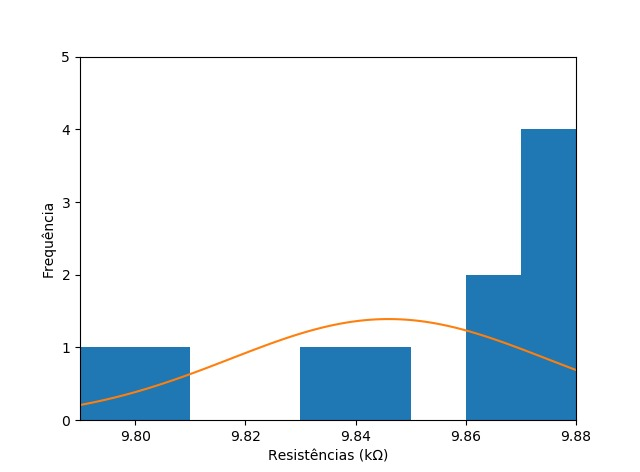
\includegraphics[scale= 0.5]{0.jpg}
                \caption{Histograma para as Resistências de 10 k$\Omega$}
                \label{fig:my_label6}
            \end{figure}
            
            \begin{figure}[H]
                \centering
                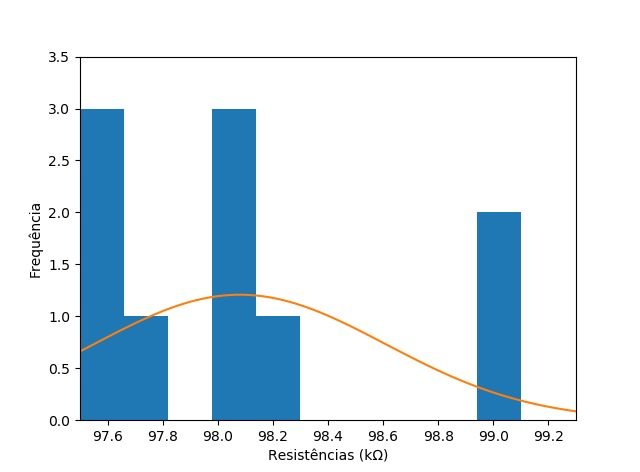
\includegraphics[scale= 0.5]{1.jpg}
                \caption{Histograma para as Resistências de 100 k$\Omega$}
                \label{fig:my_label7}
            \end{figure}
            
            
            \section{Avaliação da Rede Elétrica}
    
                \begin{table}[H]
                    \centering
                    % distancia entre a linha e o texto
                    {\renewcommand\arraystretch{1.25}
                    \caption{Valores da tensão da rede}
                    \label{rede}
                    \begin{tabular}{ l l l }
                        \cline{1-1}\cline{2-2}\cline{3-3}  
                            \multicolumn{1}{|p{3.033cm}|}{Analógico (V) \centering } &
                            \multicolumn{1}{p{2.267cm}|}{Digital (V) \centering } &
                            \multicolumn{1}{p{4.217cm}|}{True RMS (V) \centering }
                      \\  
                        \cline{1-1}\cline{2-2}\cline{3-3}  
                            \multicolumn{1}{|p{3.033cm}|}{226 \centering } &
                            \multicolumn{1}{p{2.267cm}|}{210 \centering } &
                            \multicolumn{1}{p{4.217cm}|}{214,6 \centering }
                      \\  
                        \cline{1-1}\cline{2-2}\cline{3-3}  
                            \multicolumn{1}{|p{3.033cm}|}{225 \centering } &
                            \multicolumn{1}{p{2.267cm}|}{209 \centering } &
                            \multicolumn{1}{p{4.217cm}|}{211,5 \centering }
                      \\  
                        \cline{1-1}\cline{2-2}\cline{3-3}  
                            \multicolumn{1}{|p{3.033cm}|}{225 \centering } &
                            \multicolumn{1}{p{2.267cm}|}{212 \centering } &
                            \multicolumn{1}{p{4.217cm}|}{212,8 \centering }
                      \\  
                        \cline{1-1}\cline{2-2}\cline{3-3}  
                            \multicolumn{1}{|p{3.033cm}|}{224 \centering } &
                            \multicolumn{1}{p{2.267cm}|}{208 \centering } &
                            \multicolumn{1}{p{4.217cm}|}{212,5 \centering }
                      \\  
                        \cline{1-1}\cline{2-2}\cline{3-3}  
                            \multicolumn{1}{|p{3.033cm}|}{223 \centering } &
                            \multicolumn{1}{p{2.267cm}|}{210 \centering } &
                            \multicolumn{1}{p{4.217cm}|}{211,8 \centering }
                      \\  
                        \cline{1-1}\cline{2-2}\cline{3-3}  
                            \multicolumn{1}{|p{3.033cm}|}{222 \centering } &
                            \multicolumn{1}{p{2.267cm}|}{213 \centering } &
                            \multicolumn{1}{p{4.217cm}|}{213,6 \centering }
                      \\  
                        \cline{1-1}\cline{2-2}\cline{3-3}  
                            \multicolumn{1}{|p{3.033cm}|}{224 \centering } &
                            \multicolumn{1}{p{2.267cm}|}{214 \centering } &
                            \multicolumn{1}{p{4.217cm}|}{214,5 \centering }
                      \\  
                        \cline{1-1}\cline{2-2}\cline{3-3}  
                            \multicolumn{1}{|p{3.033cm}|}{226 \centering } &
                            \multicolumn{1}{p{2.267cm}|}{211 \centering } &
                            \multicolumn{1}{p{4.217cm}|}{216,2 \centering }
                      \\  
                        \cline{1-1}\cline{2-2}\cline{3-3}  
                            \multicolumn{1}{|p{3.033cm}|}{226 \centering } &
                            \multicolumn{1}{p{2.267cm}|}{215 \centering } &
                            \multicolumn{1}{p{4.217cm}|}{213,4 \centering }
                      \\  
                        \cline{1-1}\cline{2-2}\cline{3-3}  
                            \multicolumn{1}{|p{3.033cm}|}{226 \centering } &
                            \multicolumn{1}{p{2.267cm}|}{213 \centering } &
                            \multicolumn{1}{p{4.217cm}|}{212,2 \centering }
                      \\  
                        \cline{1-1}\cline{2-2}\cline{3-3}  
                            \multicolumn{1}{|p{3.033cm}|}{226 \centering } &
                            \multicolumn{1}{p{2.267cm}|}{215 \centering } &
                            \multicolumn{1}{p{4.217cm}|}{213,5 \centering }
                    \\
                         \cline{1-1}\cline{2-2}\cline{3-3}  
                            \multicolumn{1}{|p{3.033cm}|}{226 \centering } &
                            \multicolumn{1}{p{2.267cm}|}{214 \centering } &
                            \multicolumn{1}{p{4.217cm}|}{214,3 \centering }
                    \\        
                         \cline{1-1}\cline{2-2}\cline{3-3}  
                            \multicolumn{1}{|p{3.033cm}|}{224 \centering } &
                            \multicolumn{1}{p{2.267cm}|}{213 \centering } &
                            \multicolumn{1}{p{4.217cm}|}{212,2 \centering }
                      \\
                        \cline{1-1}\cline{2-2}\cline{3-3}  
                            \multicolumn{1}{|p{3.033cm}|}{223 \centering } &
                            \multicolumn{1}{p{2.267cm}|}{212 \centering } &
                            \multicolumn{1}{p{4.217cm}|}{212,4 \centering }
                        \\
                      \cline{1-1}\cline{2-2}\cline{3-3}  
                            \multicolumn{1}{|p{3.033cm}|}{225 \centering } &
                            \multicolumn{1}{p{2.267cm}|}{214 \centering } &
                            \multicolumn{1}{p{4.217cm}|}{211,2 \centering }
                            \\
                        \hline
                    
                    \end{tabular} }
                \end{table}
                \tab Com a Tabela \ref{rede} dos valores de tensão medidos pelos três multímetros diferentes em paralelo, foi possível elaborar a Tabela $5.3$ que representa a média dos valores nominais e o erro relativo.
                
                \begin{table}[H]
                    \centering
                    \label{oi}
                    % distancia entre a linha e o texto
                    {\renewcommand\arraystretch{1.25}
                    \caption{Análise estatística dos valores de tensão da rede}
                    \begin{tabular}{ l l l l }
                        \cline{1-1}\cline{2-2}\cline{3-3}\cline{4-4}  
                            \multicolumn{1}{|p{3.033cm}|}{$\star$  \centering } &
                            \multicolumn{1}{p{3.033cm}|}{Analógico \centering } &
                            \multicolumn{1}{p{2.267cm}|}{Digital \centering } &
                            \multicolumn{1}{p{4.217cm}|}{True RMS \centering }
                      \\  
                        \cline{1-1}\cline{2-2}\cline{3-3}\cline{4-4}  
                            \multicolumn{1}{|p{3.033cm}|}{Média (V) \centering } &
                            \multicolumn{1}{p{3.033cm}|}{225 \centering } &
                            \multicolumn{1}{p{2.267cm}|}{212 \centering } &
                            \multicolumn{1}{p{4.217cm}|}{213,3 \centering }
                          \\  
                        \cline{1-1}\cline{2-2}\cline{3-3}\cline{4-4}  
                            \multicolumn{1}{|p{3.033cm}|}{Erro (\%) \centering } &
                            \multicolumn{1}{p{3.033cm}|}{2 \centering } &
                            \multicolumn{1}{p{2.267cm}|}{4 \centering } &
                            \multicolumn{1}{p{4.217cm}|}{3,0 \centering }
                          \\  
                        \hline
                    
                    \end{tabular} }
                \end{table} \\~\\
                \tab Para uma melhor visualização estatística dos valores apresentados nas tabelas anteriores, foram elaborados os três histogramas a seguir, onde cada histograma representa a análise estatística de um multímetro diferente.

                \begin{figure}[H]
                    \centering
                    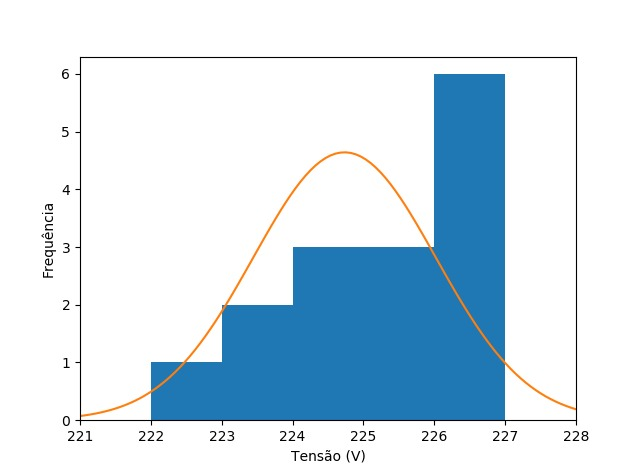
\includegraphics[scale= 0.5]{2.jpg}
                    \caption{Histograma da Avaliação da Rede pelo Multímetro Analógico}
                    \label{fig:my_labe8}
                \end{figure}
                
                 \begin{figure}[H]
                    \centering
                    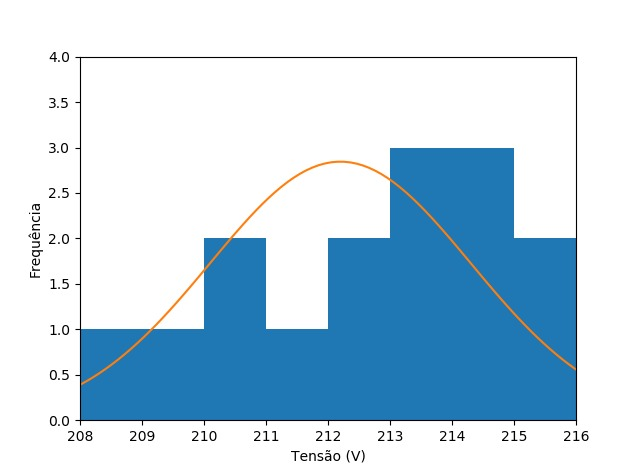
\includegraphics[scale= 0.5]{3.jpg}
                    \caption{Histograma da Avaliação da Rede pelo Multímetro Digital}
                    \label{fig:my_labe9}
                \end{figure}
                
                 \begin{figure}[H]
                    \centering
                    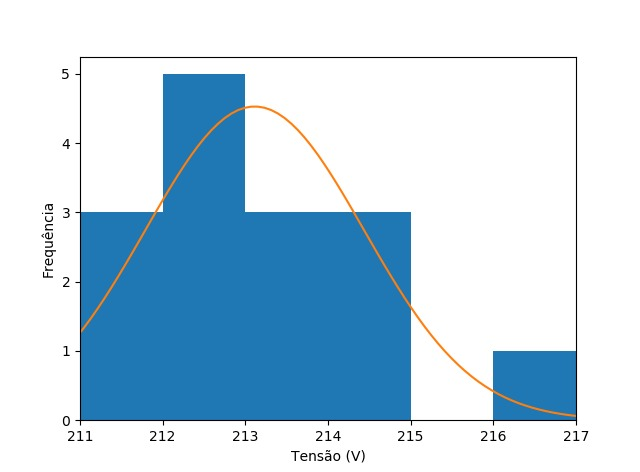
\includegraphics[scale= 0.5]{4.jpg}
                    \caption{Histograma da Avaliação da Rede pelo Multímetro True RMS}
                    \label{fig:my_labe10}
                \end{figure}

            \section{Avaliação dos Instrumentos de Medição}
			    \tab Os valores obtidos nas tabelas a seguir são os valores \textit{RMS} para ondas senoidal, quadrada e triangular.
            


                % ######## init table ########
                \begin{table}[H]
                    \centering
                    % distancia entre a linha e o texto
                    {\renewcommand\arraystretch{1.25}
                    \caption{Análise estatística dos valores de tensão no regime senoidal}
                    \begin{tabular}{ l l l l l l l l l l }
                        \cline{1-1}\cline{2-2}\cline{3-3}\cline{4-4}\cline{5-5}\cline{6-6}\cline{7-7}\cline{8-8}\cline{9-9}\cline{10-10}  
                            \multicolumn{1}{|p{3.033cm}|}{{  \centering }} &
                            \multicolumn{3}{p{3.883cm}|}{\centering \ \ \ \ \ \ 1 V  } &
                            \multicolumn{3}{p{3.117cm}|}{\ \ \ \ \ \ \ \ \ \ \ 1,5  V \centering } &
                            \multicolumn{3}{p{2.733cm}|}{\ \ \ \ \ \ \ \ \ \ \ \ 2 V \centering }
                      \\  
                        \cline{2-2}\cline{3-3}\cline{4-4}\cline{5-5}\cline{6-6}\cline{7-7}\cline{8-8}\cline{9-9}\cline{10-10}  
                            \multicolumn{1}{|p{1.0cm}|}{} &
                            \multicolumn{1}{p{1.367cm}|}{60 Hz \centering } &
                            \multicolumn{1}{p{1.333cm}|}{600 Hz \centering } &
                            \multicolumn{1}{p{1.000cm}|}{6 kHz \centering } &
                            \multicolumn{1}{p{1.350cm}|}{60 Hz \centering } &
                            \multicolumn{1}{p{1.050cm}|}{600 Hz \centering } &
                            \multicolumn{1}{p{0.983cm}|}{6 kHz \centering } &
                            \multicolumn{1}{p{1.350cm}|}{60 Hz \centering } &
                            \multicolumn{1}{p{1.050cm}|}{600 Hz \centering } &
                            \multicolumn{1}{p{0.933cm}|}{6 kHz \centering }
                      \\  
                        \cline{1-1}\cline{2-2}\cline{3-3}\cline{4-4}\cline{5-5}\cline{6-6}\cline{7-7}\cline{8-8}\cline{9-9}\cline{10-10}  
                            \multicolumn{1}{|p{3.033cm}|}{Analógico (Vrms) \centering } &
                            \multicolumn{1}{p{1.367cm}|}{0,601 \centering } &
                            \multicolumn{1}{p{1.333cm}|}{0,588 \centering } &
                            \multicolumn{1}{p{1.000cm}|}{0,611 \centering } &
                            \multicolumn{1}{p{1.350cm}|}{0,901 \centering } &
                            \multicolumn{1}{p{1.050cm}|}{0,882 \centering } &
                            \multicolumn{1}{p{0.983cm}|}{0,915 \centering } &
                            \multicolumn{1}{p{0.783cm}|}{1,178 \centering } &
                            \multicolumn{1}{p{0.933cm}|}{1,192 \centering } &
                            \multicolumn{1}{p{0.933cm}|}{1,202 \centering }
                      \\  
                        \cline{1-1}\cline{2-2}\cline{3-3}\cline{4-4}\cline{5-5}\cline{6-6}\cline{7-7}\cline{8-8}\cline{9-9}\cline{10-10}  
                            \multicolumn{1}{|p{3.033cm}|}{Digital (Vrms) \centering } &
                            \multicolumn{1}{p{1.367cm}|}{0,693 \centering } &
                            \multicolumn{1}{p{1.333cm}|}{0,692 \centering } &
                            \multicolumn{1}{p{1.000cm}|}{0,798 \centering } &
                            \multicolumn{1}{p{1.350cm}|}{1,040 \centering } &
                            \multicolumn{1}{p{1.050cm}|}{1,027 \centering } &
                            \multicolumn{1}{p{0.983cm}|}{1,200 \centering } &
                            \multicolumn{1}{p{0.783cm}|}{1,411 \centering } &
                            \multicolumn{1}{p{0.933cm}|}{1,401 \centering } &
                            \multicolumn{1}{p{0.933cm}|}{1,322 \centering }
                      \\  
                        \cline{1-1}\cline{2-2}\cline{3-3}\cline{4-4}\cline{5-5}\cline{6-6}\cline{7-7}\cline{8-8}\cline{9-9}\cline{10-10}  
                            \multicolumn{1}{|p{3.033cm}|}{True RMS (Vrms) \centering } &
                            \multicolumn{1}{p{1.367cm}|}{0,697 \centering } &
                            \multicolumn{1}{p{1.333cm}|}{0,693 \centering } &
                            \multicolumn{1}{p{1.000cm}|}{0,665 \centering } &
                            \multicolumn{1}{p{1.350cm}|}{1,035 \centering } &
                            \multicolumn{1}{p{1.050cm}|}{1,032 \centering } &
                            \multicolumn{1}{p{0.983cm}|}{0,997 \centering } &
                            \multicolumn{1}{p{0.783cm}|}{1,400 \centering } &
                            \multicolumn{1}{p{0.933cm}|}{1,391 \centering } &
                            \multicolumn{1}{p{0.933cm}|}{1,320 \centering }
                      \\  
                        \hline
                    
                    \end{tabular} }
                \end{table}
                \begin{table}[H]
                    \centering
                    % distancia entre a linha e o texto
                    {\renewcommand\arraystretch{1.25}
                    \caption{Análise estatística dos valores de tensão no regime quadrado}
                    \begin{tabular}{ l l l l l l l l l l }
                        \cline{1-1}\cline{2-2}\cline{3-3}\cline{4-4}\cline{5-5}\cline{6-6}\cline{7-7}\cline{8-8}\cline{9-9}\cline{10-10}  
                            \multicolumn{1}{|p{3.033cm}|}{{  \centering }} &
                            \multicolumn{3}{p{3.883cm}|}{\centering \ \ \ \ \ \ 1 V  } &
                            \multicolumn{3}{p{3.117cm}|}{\ \ \ \ \ \ \ \ \ \ \ 1,5  V \centering } &
                            \multicolumn{3}{p{2.733cm}|}{\ \ \ \ \ \ \ \ \ \ \ \ 2 V \centering }
                      \\  
                        \cline{2-2}\cline{3-3}\cline{4-4}\cline{5-5}\cline{6-6}\cline{7-7}\cline{8-8}\cline{9-9}\cline{10-10}  
                            \multicolumn{1}{|p{1.0cm}|}{} &
                            \multicolumn{1}{p{1.367cm}|}{60 Hz \centering } &
                            \multicolumn{1}{p{1.333cm}|}{600 Hz \centering } &
                            \multicolumn{1}{p{1.000cm}|}{6 kHz \centering } &
                            \multicolumn{1}{p{1.350cm}|}{60 Hz \centering } &
                            \multicolumn{1}{p{1.050cm}|}{600 Hz \centering } &
                            \multicolumn{1}{p{0.983cm}|}{6 kHz \centering } &
                            \multicolumn{1}{p{1.350cm}|}{60 Hz \centering } &
                            \multicolumn{1}{p{1.050cm}|}{600 Hz \centering } &
                            \multicolumn{1}{p{0.933cm}|}{6 kHz \centering }
                      \\  
                        \cline{1-1}\cline{2-2}\cline{3-3}\cline{4-4}\cline{5-5}\cline{6-6}\cline{7-7}\cline{8-8}\cline{9-9}\cline{10-10}  
                            \multicolumn{1}{|p{3.033cm}|}{Analógico ($V_{RMS}$) \centering } &
                            \multicolumn{1}{p{1.367cm}|}{0,801 \centering } &
                            \multicolumn{1}{p{1.333cm}|}{0,899 \centering } &
                            \multicolumn{1}{p{1.000cm}|}{0,698 \centering } &
                            \multicolumn{1}{p{1.350cm}|}{1,501 \centering } &
                            \multicolumn{1}{p{1.050cm}|}{1,240 \centering } &
                            \multicolumn{1}{p{0.983cm}|}{1,410 \centering } &
                            \multicolumn{1}{p{0.783cm}|}{1,801 \centering } &
                            \multicolumn{1}{p{0.933cm}|}{1,802 \centering } &
                            \multicolumn{1}{p{0.933cm}|}{1,600 \centering }
                      \\  
                        \cline{1-1}\cline{2-2}\cline{3-3}\cline{4-4}\cline{5-5}\cline{6-6}\cline{7-7}\cline{8-8}\cline{9-9}\cline{10-10}  
                            \multicolumn{1}{|p{3.033cm}|}{Digital ($V_{RMS}$) \centering } &
                            \multicolumn{1}{p{1.367cm}|}{1,032 \centering } &
                            \multicolumn{1}{p{1.333cm}|}{1,090 \centering } &
                            \multicolumn{1}{p{1.000cm}|}{1,070 \centering } &
                            \multicolumn{1}{p{1.350cm}|}{1,600 \centering } &
                            \multicolumn{1}{p{1.050cm}|}{1,619 \centering } &
                            \multicolumn{1}{p{0.983cm}|}{2,050 \centering } &
                            \multicolumn{1}{p{0.783cm}|}{2,088 \centering } &
                            \multicolumn{1}{p{0.933cm}|}{2,140 \centering } &
                            \multicolumn{1}{p{0.933cm}|}{2,633 \centering }
                      \\  
                        \cline{1-1}\cline{2-2}\cline{3-3}\cline{4-4}\cline{5-5}\cline{6-6}\cline{7-7}\cline{8-8}\cline{9-9}\cline{10-10}  
                            \multicolumn{1}{|p{3.033cm}|}{True RMS ($V_{RMS}$) \centering } &
                            \multicolumn{1}{p{1.367cm}|}{0,980 \centering } &
                            \multicolumn{1}{p{1.333cm}|}{0,970 \centering } &
                            \multicolumn{1}{p{1.000cm}|}{0,809 \centering } &
                            \multicolumn{1}{p{1.350cm}|}{1,460 \centering } &
                            \multicolumn{1}{p{1.050cm}|}{1,415 \centering } &
                            \multicolumn{1}{p{0.983cm}|}{1,224 \centering } &
                            \multicolumn{1}{p{0.783cm}|}{1,040 \centering } &
                            \multicolumn{1}{p{0.933cm}|}{1,030 \centering } &
                            \multicolumn{1}{p{0.933cm}|}{0,988 \centering }
                      \\  
                        \hline
                    
                    \end{tabular} }
                \end{table}
                
                \begin{table}[H]
                    \centering
                    % distancia entre a linha e o texto
                    {\renewcommand\arraystretch{1.25}
                    \caption{Análise estatística dos valores de tensão no regime triangular}
                    \begin{tabular}{ l l l l l l l l l l }
                        \cline{1-1}\cline{2-2}\cline{3-3}\cline{4-4}\cline{5-5}\cline{6-6}\cline{7-7}\cline{8-8}\cline{9-9}\cline{10-10}  
                            \multicolumn{1}{|p{3.033cm}|}{{  \centering }} &
                            \multicolumn{3}{p{3.883cm}|}{\centering \ \ \ \ \ \ 1 V  } &
                            \multicolumn{3}{p{3.117cm}|}{\ \ \ \ \ \ \ \ \ \ \ 1,5  V \centering } &
                            \multicolumn{3}{p{2.733cm}|}{\ \ \ \ \ \ \ \ \ \ \ \ 2 V \centering }
                      \\  
                        \cline{2-2}\cline{3-3}\cline{4-4}\cline{5-5}\cline{6-6}\cline{7-7}\cline{8-8}\cline{9-9}\cline{10-10}  
                            \multicolumn{1}{|p{1.0cm}|}{} &
                            \multicolumn{1}{p{1.367cm}|}{60 Hz \centering } &
                            \multicolumn{1}{p{1.333cm}|}{600 Hz \centering } &
                            \multicolumn{1}{p{1.000cm}|}{6 kHz \centering } &
                            \multicolumn{1}{p{1.350cm}|}{60 Hz \centering } &
                            \multicolumn{1}{p{1.050cm}|}{600 Hz \centering } &
                            \multicolumn{1}{p{0.983cm}|}{6 kHz \centering } &
                            \multicolumn{1}{p{1.350cm}|}{60 Hz \centering } &
                            \multicolumn{1}{p{1.050cm}|}{600 Hz \centering } &
                            \multicolumn{1}{p{0.933cm}|}{6 kHz \centering }
                      \\  
                        \cline{1-1}\cline{2-2}\cline{3-3}\cline{4-4}\cline{5-5}\cline{6-6}\cline{7-7}\cline{8-8}\cline{9-9}\cline{10-10}  
                            \multicolumn{1}{|p{3.033cm}|}{Analógico ($V_{RMS}$) \centering } &
                            \multicolumn{1}{p{1.367cm}|}{0,401 \centering } &
                            \multicolumn{1}{p{1.333cm}|}{0,402 \centering } &
                            \multicolumn{1}{p{1.000cm}|}{0,402 \centering } &
                            \multicolumn{1}{p{1.350cm}|}{0,702 \centering } &
                            \multicolumn{1}{p{1.050cm}|}{0,705 \centering } &
                            \multicolumn{1}{p{0.983cm}|}{0,705 \centering } &
                            \multicolumn{1}{p{0.783cm}|}{0,902 \centering } &
                            \multicolumn{1}{p{0.933cm}|}{0,890 \centering } &
                            \multicolumn{1}{p{0.933cm}|}{0,895 \centering }
                      \\  
                        \cline{1-1}\cline{2-2}\cline{3-3}\cline{4-4}\cline{5-5}\cline{6-6}\cline{7-7}\cline{8-8}\cline{9-9}\cline{10-10}  
                            \multicolumn{1}{|p{3.033cm}|}{Digital ($V_{RMS}$) \centering } &
                            \multicolumn{1}{p{1.367cm}|}{0,550 \centering } &
                            \multicolumn{1}{p{1.333cm}|}{0,540 \centering } &
                            \multicolumn{1}{p{1.000cm}|}{0,621 \centering } &
                            \multicolumn{1}{p{1.350cm}|}{0,820 \centering } &
                            \multicolumn{1}{p{1.050cm}|}{0,815 \centering } &
                            \multicolumn{1}{p{0.983cm}|}{0,980 \centering } &
                            \multicolumn{1}{p{0.783cm}|}{1,122 \centering } &
                            \multicolumn{1}{p{0.933cm}|}{1,100 \centering } &
                            \multicolumn{1}{p{0.933cm}|}{1,005 \centering }
                      \\  
                        \cline{1-1}\cline{2-2}\cline{3-3}\cline{4-4}\cline{5-5}\cline{6-6}\cline{7-7}\cline{8-8}\cline{9-9}\cline{10-10}  
                            \multicolumn{1}{|p{3.033cm}|}{True RMS ($V_{RMS}$) \centering } &
                            \multicolumn{1}{p{1.367cm}|}{0,580 \centering } &
                            \multicolumn{1}{p{1.333cm}|}{0,550 \centering } &
                            \multicolumn{1}{p{1.000cm}|}{0,539 \centering } &
                            \multicolumn{1}{p{1.350cm}|}{0,882 \centering } &
                            \multicolumn{1}{p{1.050cm}|}{0,865 \centering } &
                            \multicolumn{1}{p{0.983cm}|}{0,813 \centering } &
                            \multicolumn{1}{p{0.783cm}|}{1,150 \centering } &
                            \multicolumn{1}{p{0.933cm}|}{1,140 \centering } &
                            \multicolumn{1}{p{0.933cm}|}{1,092 \centering }
                      \\  
                        \hline
                    
                    \end{tabular} }
                \end{table}
            
            \section{Avaliação do Amplificador}
                \begin{figure}[h]
                    \centering
                    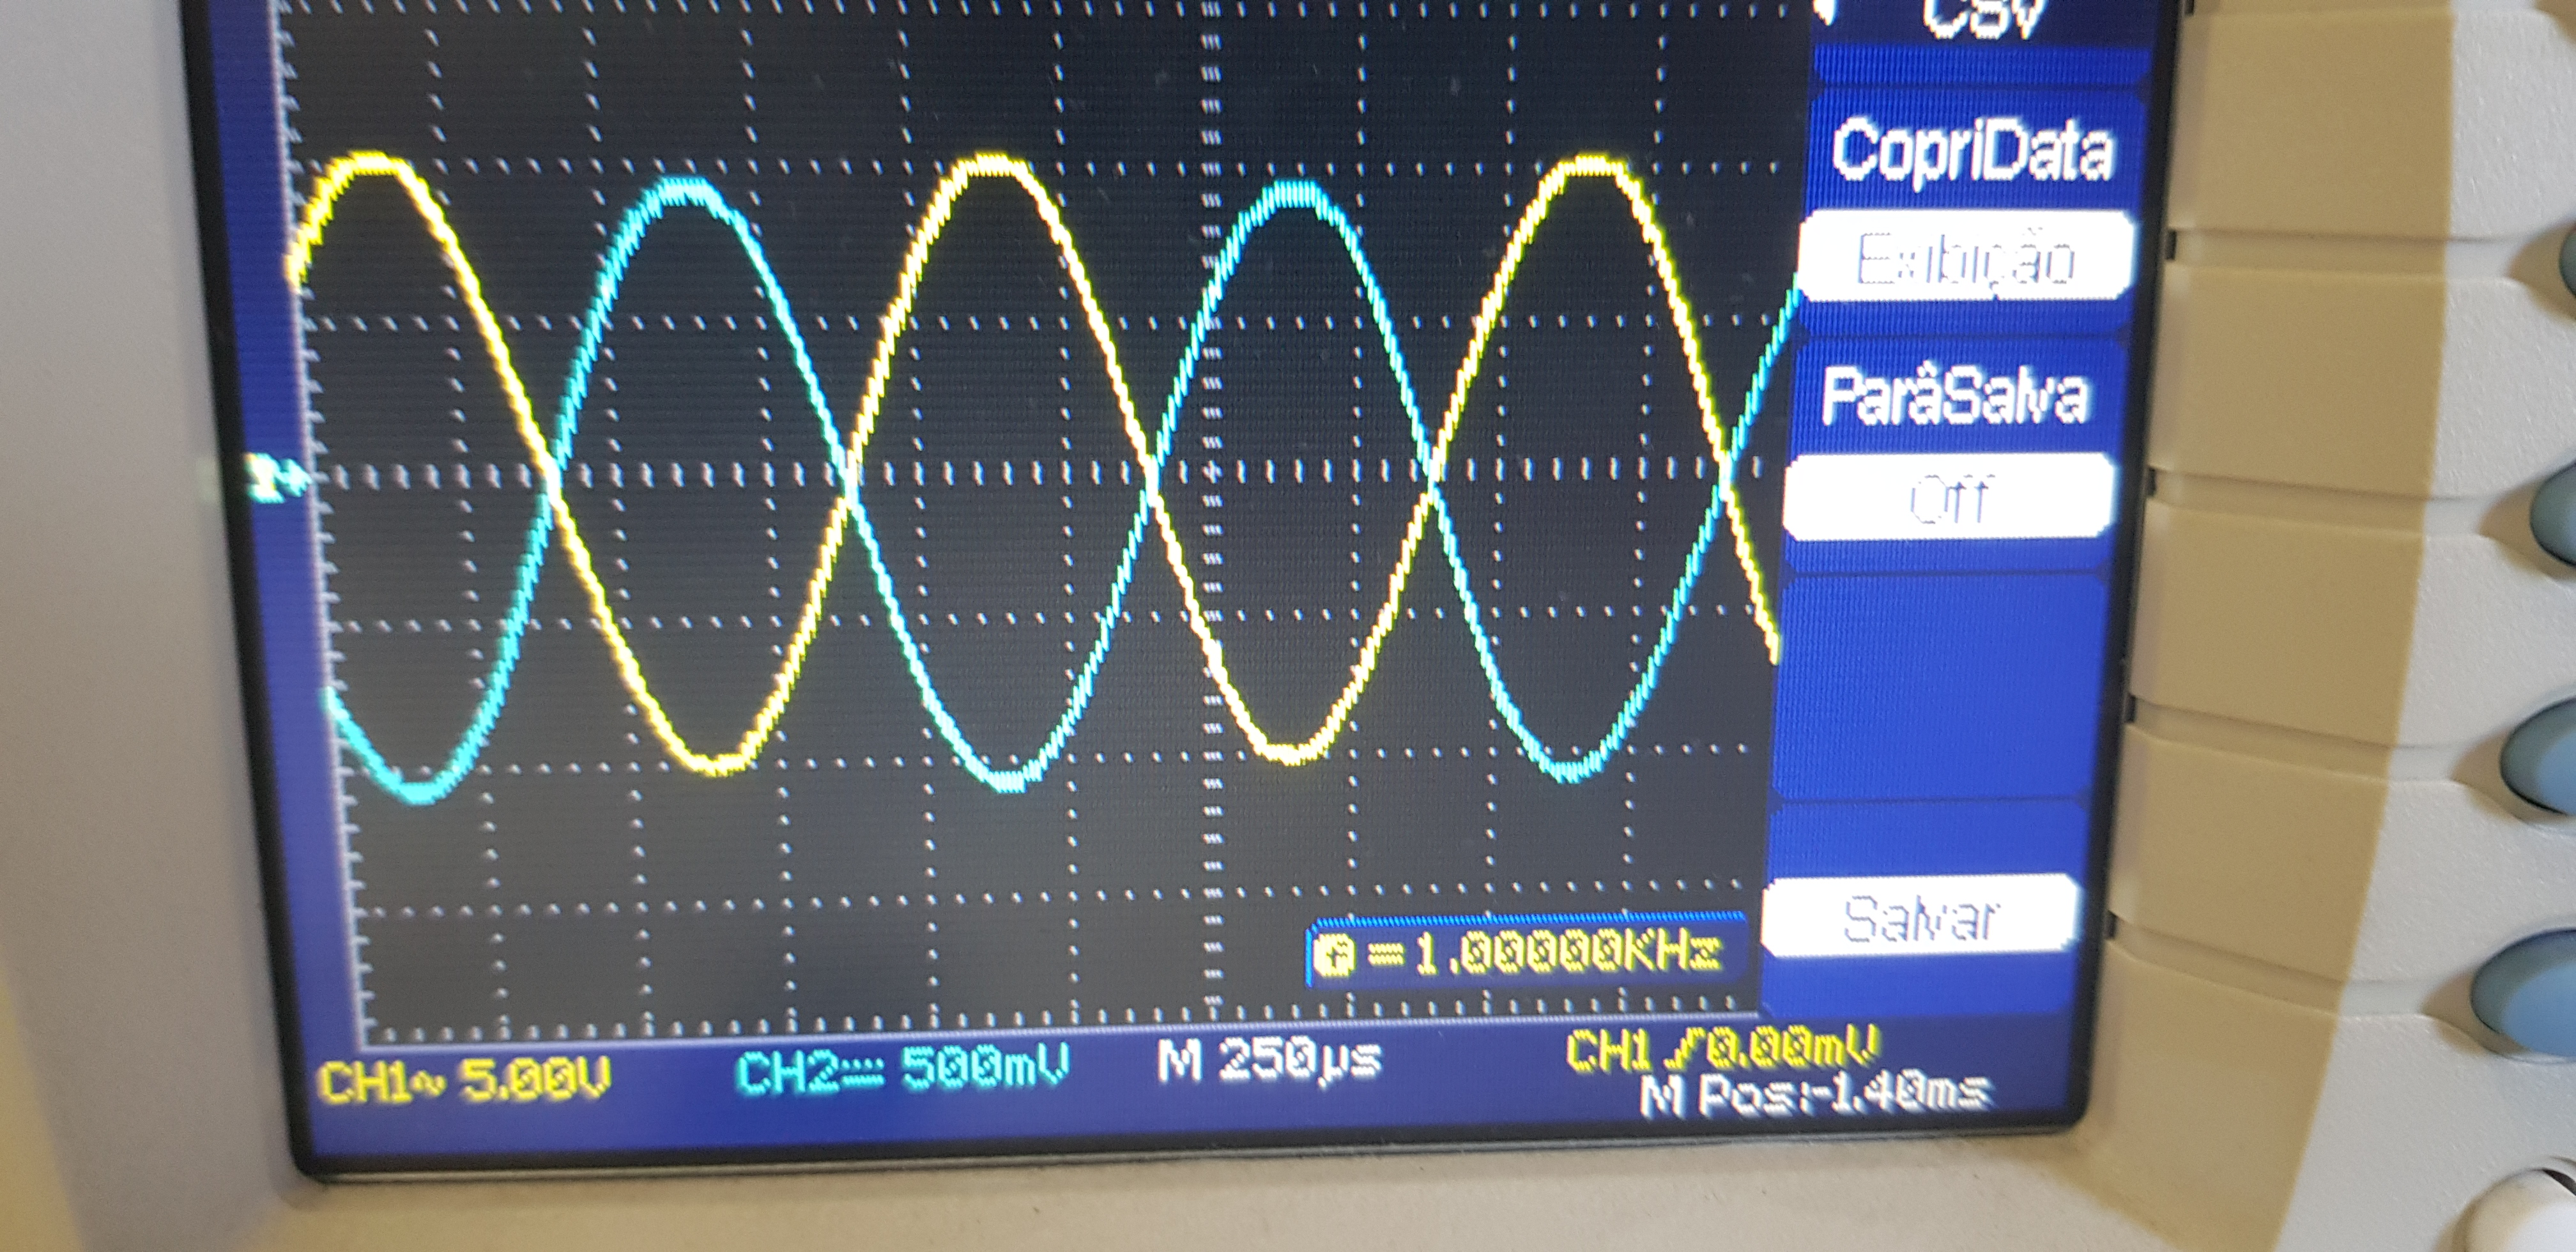
\includegraphics[scale = 0.10]{seno.jpg}
                    \caption{Amplificador Operacional - Onda Senoidal}
                    \label{seno}
                \end{figure}            
                \\~\\
                \tab É possível observar pela escala nas Figuras \ref{seno} e \ref{quadrada}, onde o Canal 1 representa a saída e o Canal 2 representa a entrada, em ambos os regimes.
                
                \begin{figure}[H]
                    \centering
                    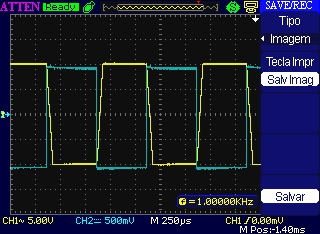
\includegraphics[scale = 1.0]{quadrado.jpg}
                    \caption{Amplificador Operacional - Onda Quadrada}
                    \label{quadrada}
                \end{figure}
            
            \section{Avaliação do Sistema}
                \tab Conforme mostra a Tabela 5.7 abaixo, foram feitas três medidas diferentes de temperatura pelo LM$35$ e pelo True RMS. Para aferir a temperatura pelo LM$35$, foi medido a tensão na saída, que é 10 vezes menor (em V) do que a temperatura (em $^0$C).
                % ######## init table ########
                \begin{table}[H]
                    \centering
                    \label{tempo}
                    % distancia entre a linha e o texto
                    {\renewcommand\arraystretch{1.25}
                    \caption{Temperaturas medidas}
                    \begin{tabular}{ l l }
                        \cline{1-1}\cline{2-2}  
                            \multicolumn{1}{|p{2.967cm}|}{LM35 ($^0$C) \centering } &
                            \multicolumn{1}{p{2.883cm}|}{True RMS ($^0$C) \centering }
                            \multicolumn{1}{p{2.883cm}|}{Erro ($\%$) \centering }
                      \\  
                        \cline{1-1}\cline{2-2}  
                            \multicolumn{1}{|p{2.967cm}|}{21,9 \centering } &
                            \multicolumn{1}{p{2.883cm}|}{21 \centering }
                            \multicolumn{1}{p{2.883cm}|}{4,28 \centering }
                      \\  
                        \cline{1-1}\cline{2-2}  
                            \multicolumn{1}{|p{2.967cm}|}{53,1 \centering } &
                            \multicolumn{1}{p{2.883cm}|}{52 \centering }
                            \multicolumn{1}{p{2.883cm}|}{2,11 \centering }
                      \\  
                        \cline{1-1}\cline{2-2}  
                            \multicolumn{1}{|p{2.967cm}|}{74,1 \centering } &
                            \multicolumn{1}{p{2.883cm}|}{71 \centering }
                            \multicolumn{1}{p{2.883cm}|}{4,36 \centering }
                      \\  
                        \hline
                    
                    \end{tabular} }
                \end{table}
                
        \chapter{Análise}
            \section{Avaliação dos Resistores}
              \\
                \tab Foi percebido que todos os resistores utilizados estavam bem abaixo da faixa de tolerância dada pelo fabricante ($5\%$), visto que tomando a tolerância de $\pm5\%$, para o resistor de $10$ k$\Omega$ significa que o menor valor possível seria $9,5$ k$\Omega$, e o maior seria $10,5$ k$\Omega$, sendo que o menor e maior resistores obtidos foram $9,79$ k$\Omega$ e $9,87$ k$\Omega$. Para $100$ k$\Omega$, os menores e maiores valores teoricamente seriam $90$ k$\Omega$ e $110$ k$\Omega$, sendo que os menores e maiores valores obtidos foram $97,6$ k$\Omega$ e $99,1$ k$\Omega$.
            
            \section{Avaliação da Rede Elétrica}
            \\
                \tab O maior e o menor valor obtidos nas medições (tomando como base o True RMS) foram $211,2$ V e $216,2$ V. Segundo os padrões da ANEEL, estes valores estão de acordo com o aceitável, que dita que os valores de tensão medidos devem ser na faixa de $208$ V a $242$ V.
                
            \section{Avaliação dos Instrumentos de Medição}
            
                \subsection{Multímetro Analógico MXT YX-360TRN}
                    \tab No que diz respeito à medição de tensão AC, o modo utilizado neste trabalho, de acordo com as especificações técnicas como mostrado na Figura \ref{data2}, o multímetro em questão tem precisão de $\pm 4\%  fs$.
                    Onde \textit{fs} é o fundo de escala, que é o valor máximo lido pelo multímetro em certa escala.
                    Para a faixa de valores medidos com o multímetro analógico, o erro médio medido foi de
                    ($18,51\pm 8,1$)\%, que condiz com o erro médio calculado de acordo com as especificações do
                    multímetro, $20\%$.
                    
                    \begin{figure}
                        \centering
                        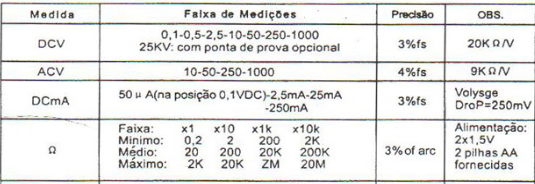
\includegraphics[scale = 1]{datasheet2.png}
                        \caption{Datasheet do Multímetro MXT YX-360TRN}
                        \label{data2}
                    \end{figure}
                    
                    
                \subsection{Multímetro Digital ET-2042C}
                    \tab No que diz respeito à medição de tensão AC, o modo utilizado neste trabalho, de acordo
                    com as especificações técnicas, o multímetro em questão tem precisão de $\pm(0.8\%.rdg+3.dgts)$. Onde a primeira parte \textit{rdg} (\textit{reading}) é variável e corresponde a uma porcentagem
                    do valor de entrada e a segunda parte \textit{dgts} (\textit{digits}) é fixa e corresponde, nesse caso, a $3$
                    vezes o dígito menos significativo da medição.
                    Para a faixa de valores medidos com o multímetro digital, o erro médio medido foi de
                    $(9,10\pm 8,62)\%$, que condiz com o erro médio calculado de acordo com as especificações do multímetro, $9,5\%$.
                    
                    \begin{figure}[H]
                        \centering
                        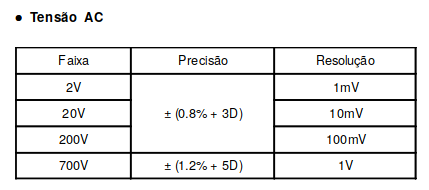
\includegraphics{datasheet3.png}
                        \caption{Datasheet do Multímetro Digital ET-2042C}
                        \label{data3}
                    \end{figure}
                \subsection{Multímetro True RMS Meterman 38XR}
                    \tab No que diz respeito à medição de tensão, de acordo com as especificações técnicas, o multímetro em questão tem precisão de $\pm(1.2\%. rdg + 10 .dgts)$ para frequências
                    entre $45$ e $500$ Hz e $(2.0\%. rdg +10. dgts)$ para frequências entre $500$ e $2$ kHz. Onde a
                    primeira parte \texit{rdg} (reading) é variável e corresponde a uma porcentagem do valor de entrada
                    e a segunda parte \texit{dgts} (digits) é fixa e corresponde, nesse caso, a 10 vezes o dígito menos significativo da medição. \\
                    \tab Para a faixa de valores medidos com o multímetro True RMS, o erro médio medido foi de
                    $(4,61\pm5,34)\%$, que condiz com o erro médio calculado de acordo com as especificações do
                    multímetro, $6,6$\%. Dentre todos os multímetros, este foi o que apresentou menor erro médio,
                    o que era esperado, uma vez que o multímetro digital e o analógico consideram uma entrada
                    AC como uma onda senoidal de baixa frequência, que implica em erros elevados quando
                    são medidas outras formas de ondas e altas frequências.
                
                    \begin{figure}[H]
                        \centering
                        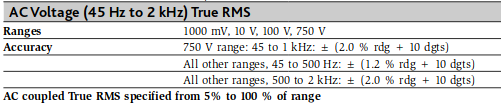
\includegraphics[scale = 1]{figura7.png}
                        \caption{Datasheet do Multímetro True RMS Meterman 38XR}
                        \label{fig:my_label}
                    \end{figure}
            \section{Avaliação do Amplificador}
                \tab Para os testes feitos com as frequências entre $0$ a aproximadamente $50$ kHz, o amplificador operacional LM$741$ mostrou-se bastante eficaz, e por isso, no caso desse projeto, onde foi trabalhado as frequências de $60$ Hz, $600$ Hz e $6$ kHz, o componente funcionou de maneira bastante satisfatória, permanecendo com seu ganho muito próximo de 10. \\
                \tab Com a simulação no \textit{Proteus}, foi possível plotar o diagrama de bode para o amplificador, nele, é perceptível a qualidade do funcionamento até valores próximos de $50$ kHz.
                
                
                \begin{figure}[H]
                    \centering
                    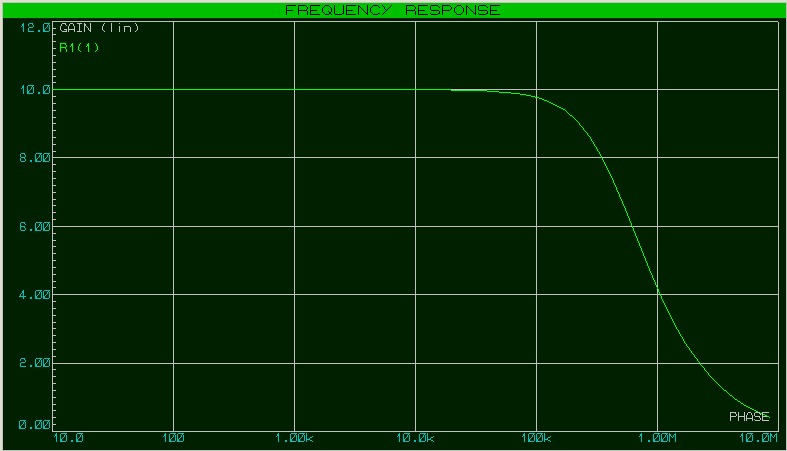
\includegraphics[scale= 0.5]{bode.jpg}
                    \caption{Diagrama de Bode para o LM$741$}
                    \label{fig:my_label}
                \end{figure}
            \section{Avaliação do LM$35$ e Sistema}
                \tab Segundo o datasheet do LM$35$ (Figura \ref{datasheet}, o sensor funciona bem entre as temperaturas de $-55^0$C e $150^0$C com uma variação de $10$mV/$^0$C.
                
                \begin{figure}[H]
                    \centering
                    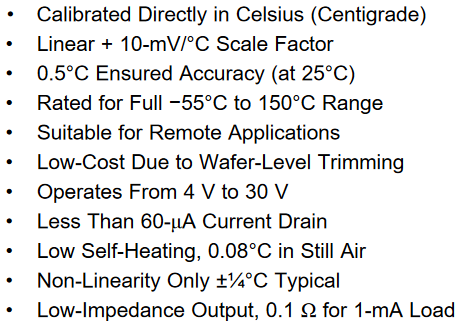
\includegraphics[scale = 0.8]{datasheet.png}
                    \caption{Datasheet do LM$35$}
                    \label{datasheet}
                \end{figure} \\
                \tab No presente projeto, tomou-se como base o multímetro True RMS para estabelecer o desvio de realidade do sistema final, disso, foi possível perceber que o erro foi aceitável diante da simplicidade da construção do aparato, bem como a forma com a qual foi medido os valores.
                
        \chapter{Conclusão}
            \tab O desenvolvimento do trabalho foi de extrema importância para a vivência prática dos conhecimentos adquiridos ao longo das aulas da disciplina de Medidas Eletromagnéticas. \\
            \tab Inicialmente verificou-se a importância de escolher corretamente quais instrumentos de medida utilizar, bem como quais elementos, tal que o projeto se aproxime o máximo da idealidade. \\
            \tab Algo bastante relevante no desenvolver do projeto foi o aprendizado relacionado a confecção de placas de circuito impresso. Durante a confecção ocorreram problemas, como: dificuldade de gravura na placa, espessura da trilha, etc. Problemas comuns de acontecer e que, com a vivência do presente projeto, foram resolvidos e absorvidos como forma de conhecimento. \\
            \tab Ocorreu também diversas vezes em que precisamos analisar especificações do fabricante, checar informações no datasheet, prática bastante importante para um engenheiro e que foi feita pela primeira vez no curso através desse projeto. \\
            \tab Por fim, apesar das imperfeições, das incertezas de medida e dos desvios de realidade, os resultados finais foram bastante próximos do esperado, de forma que o projeto foi, além de muito importante como forma de conhecimento, um produto final válido.
            
        \chapter{Anexos}
        
            \begin{figure}[H]
                \centering
                \subfloat[Visão superior]{{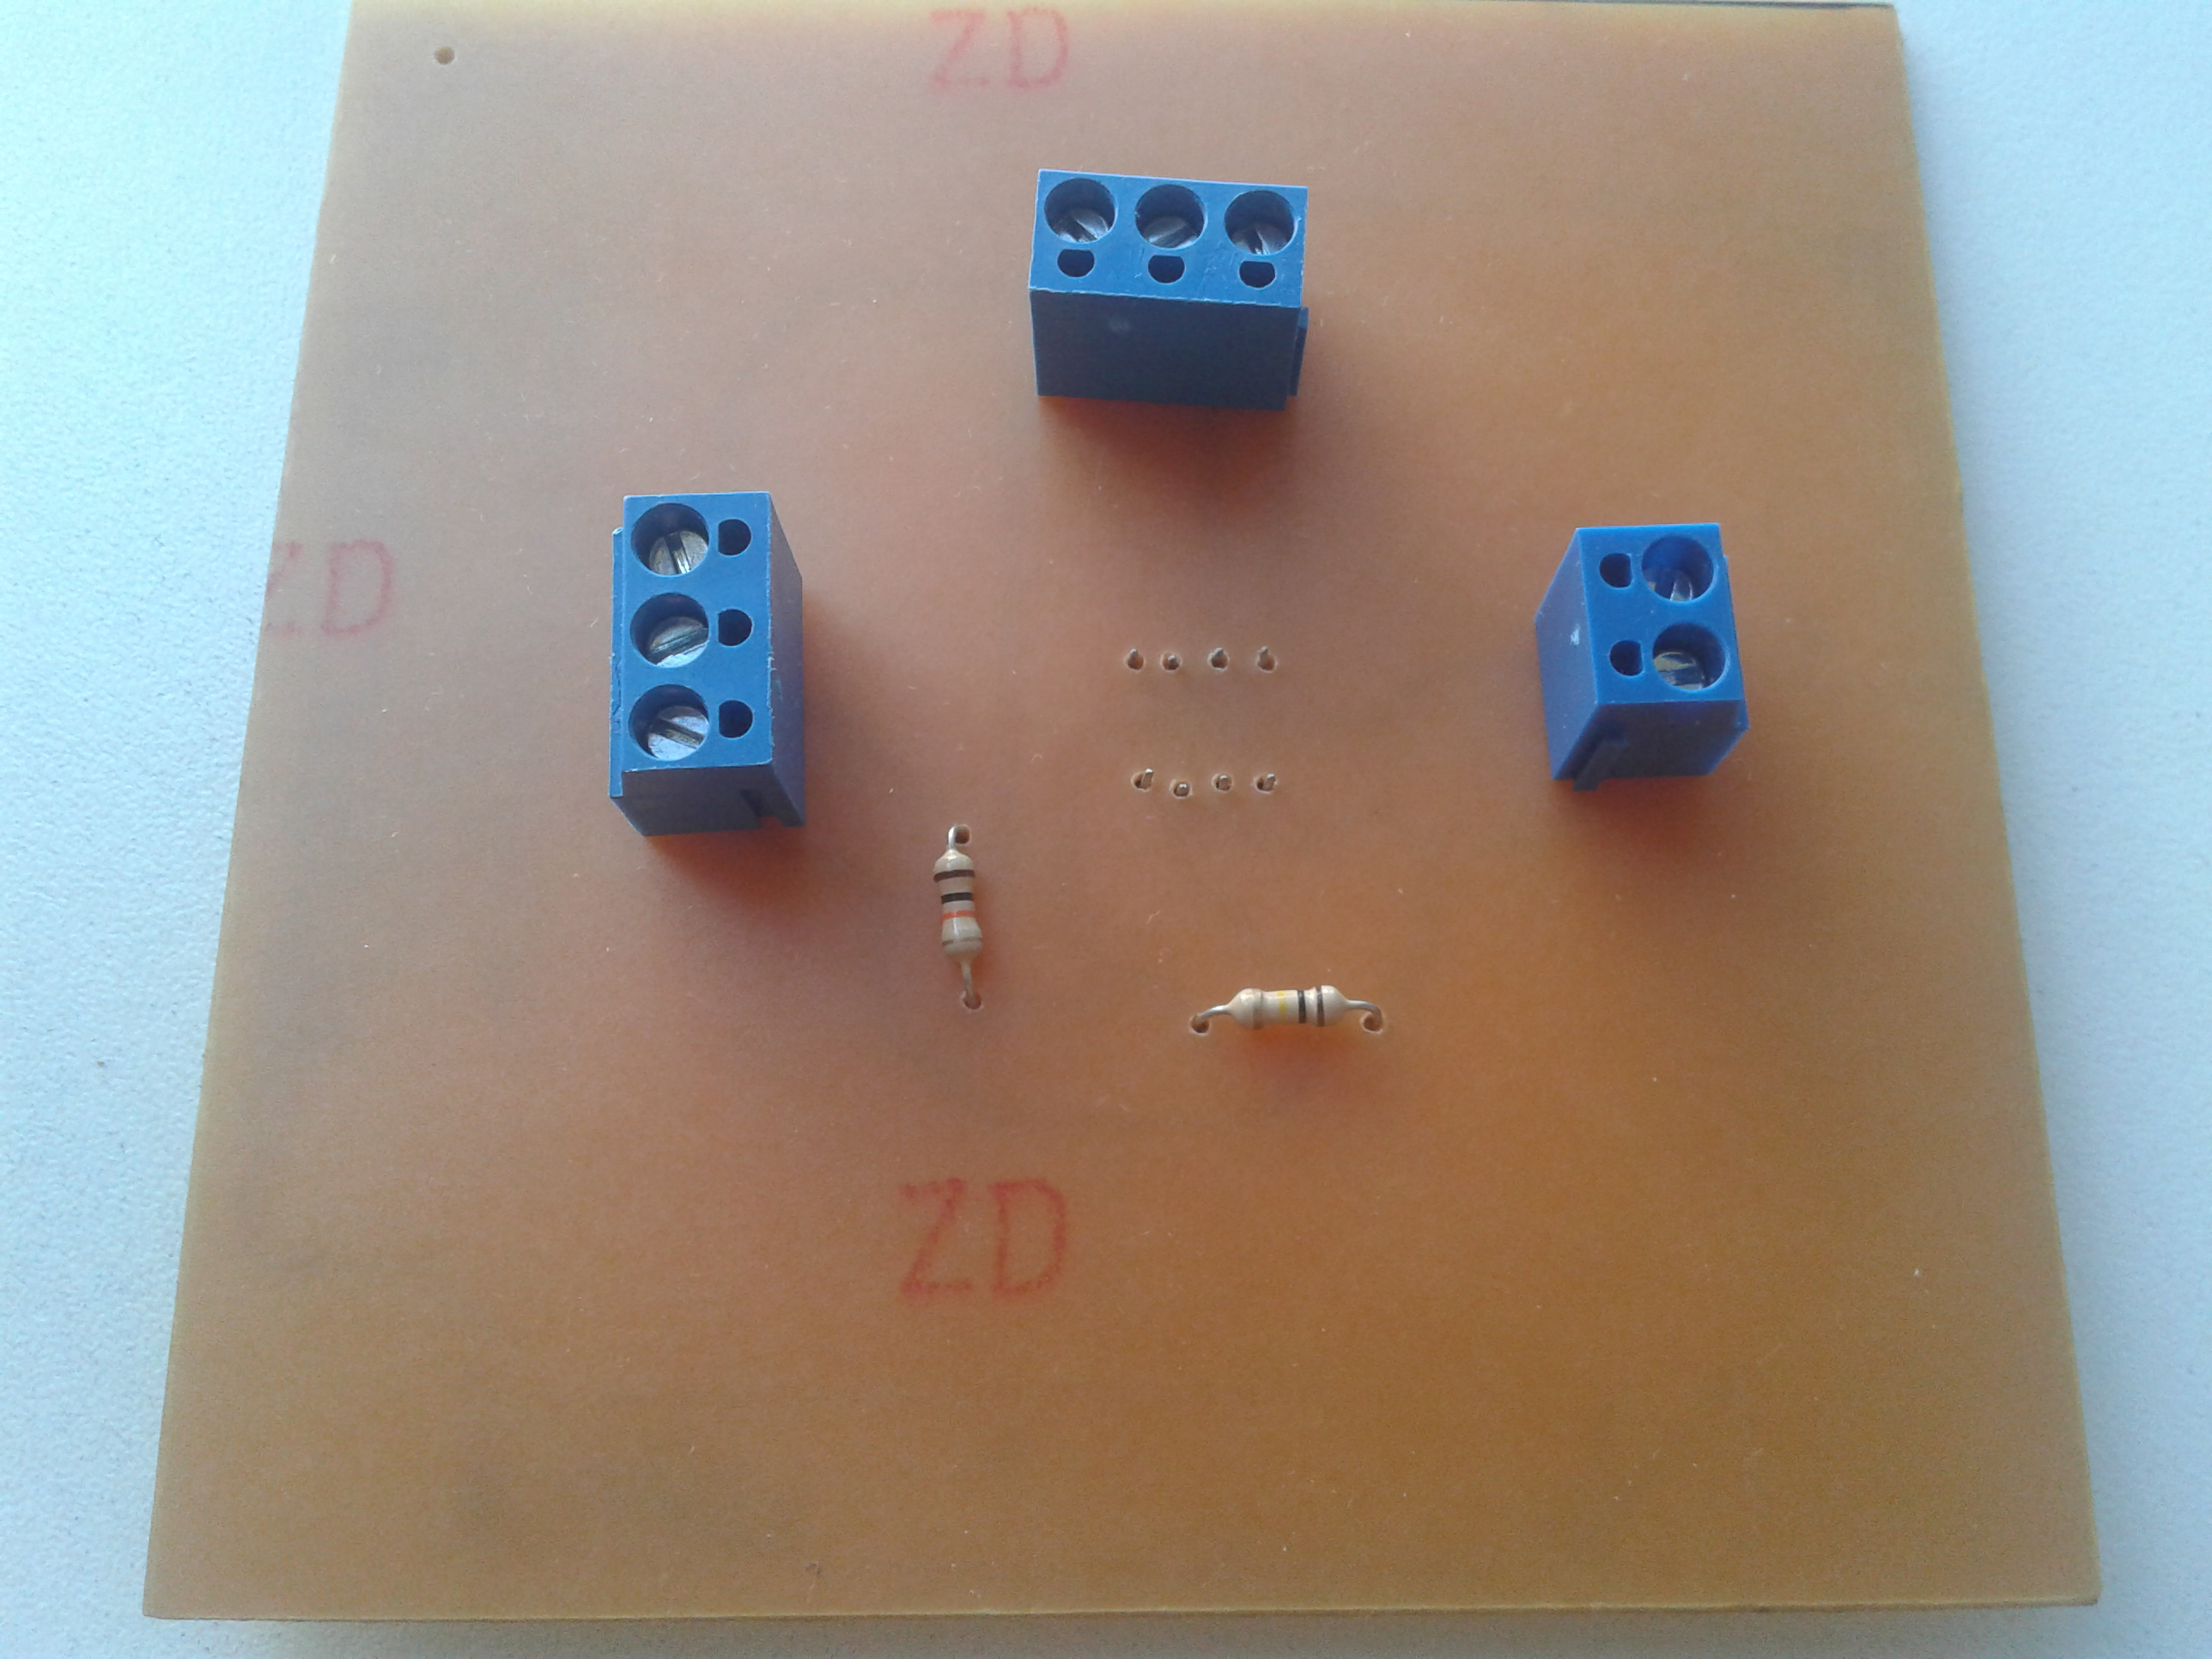
\includegraphics[width=5cm]{f1.jpg} }}%
                \qquad
                \subfloat[Visão inferior]{{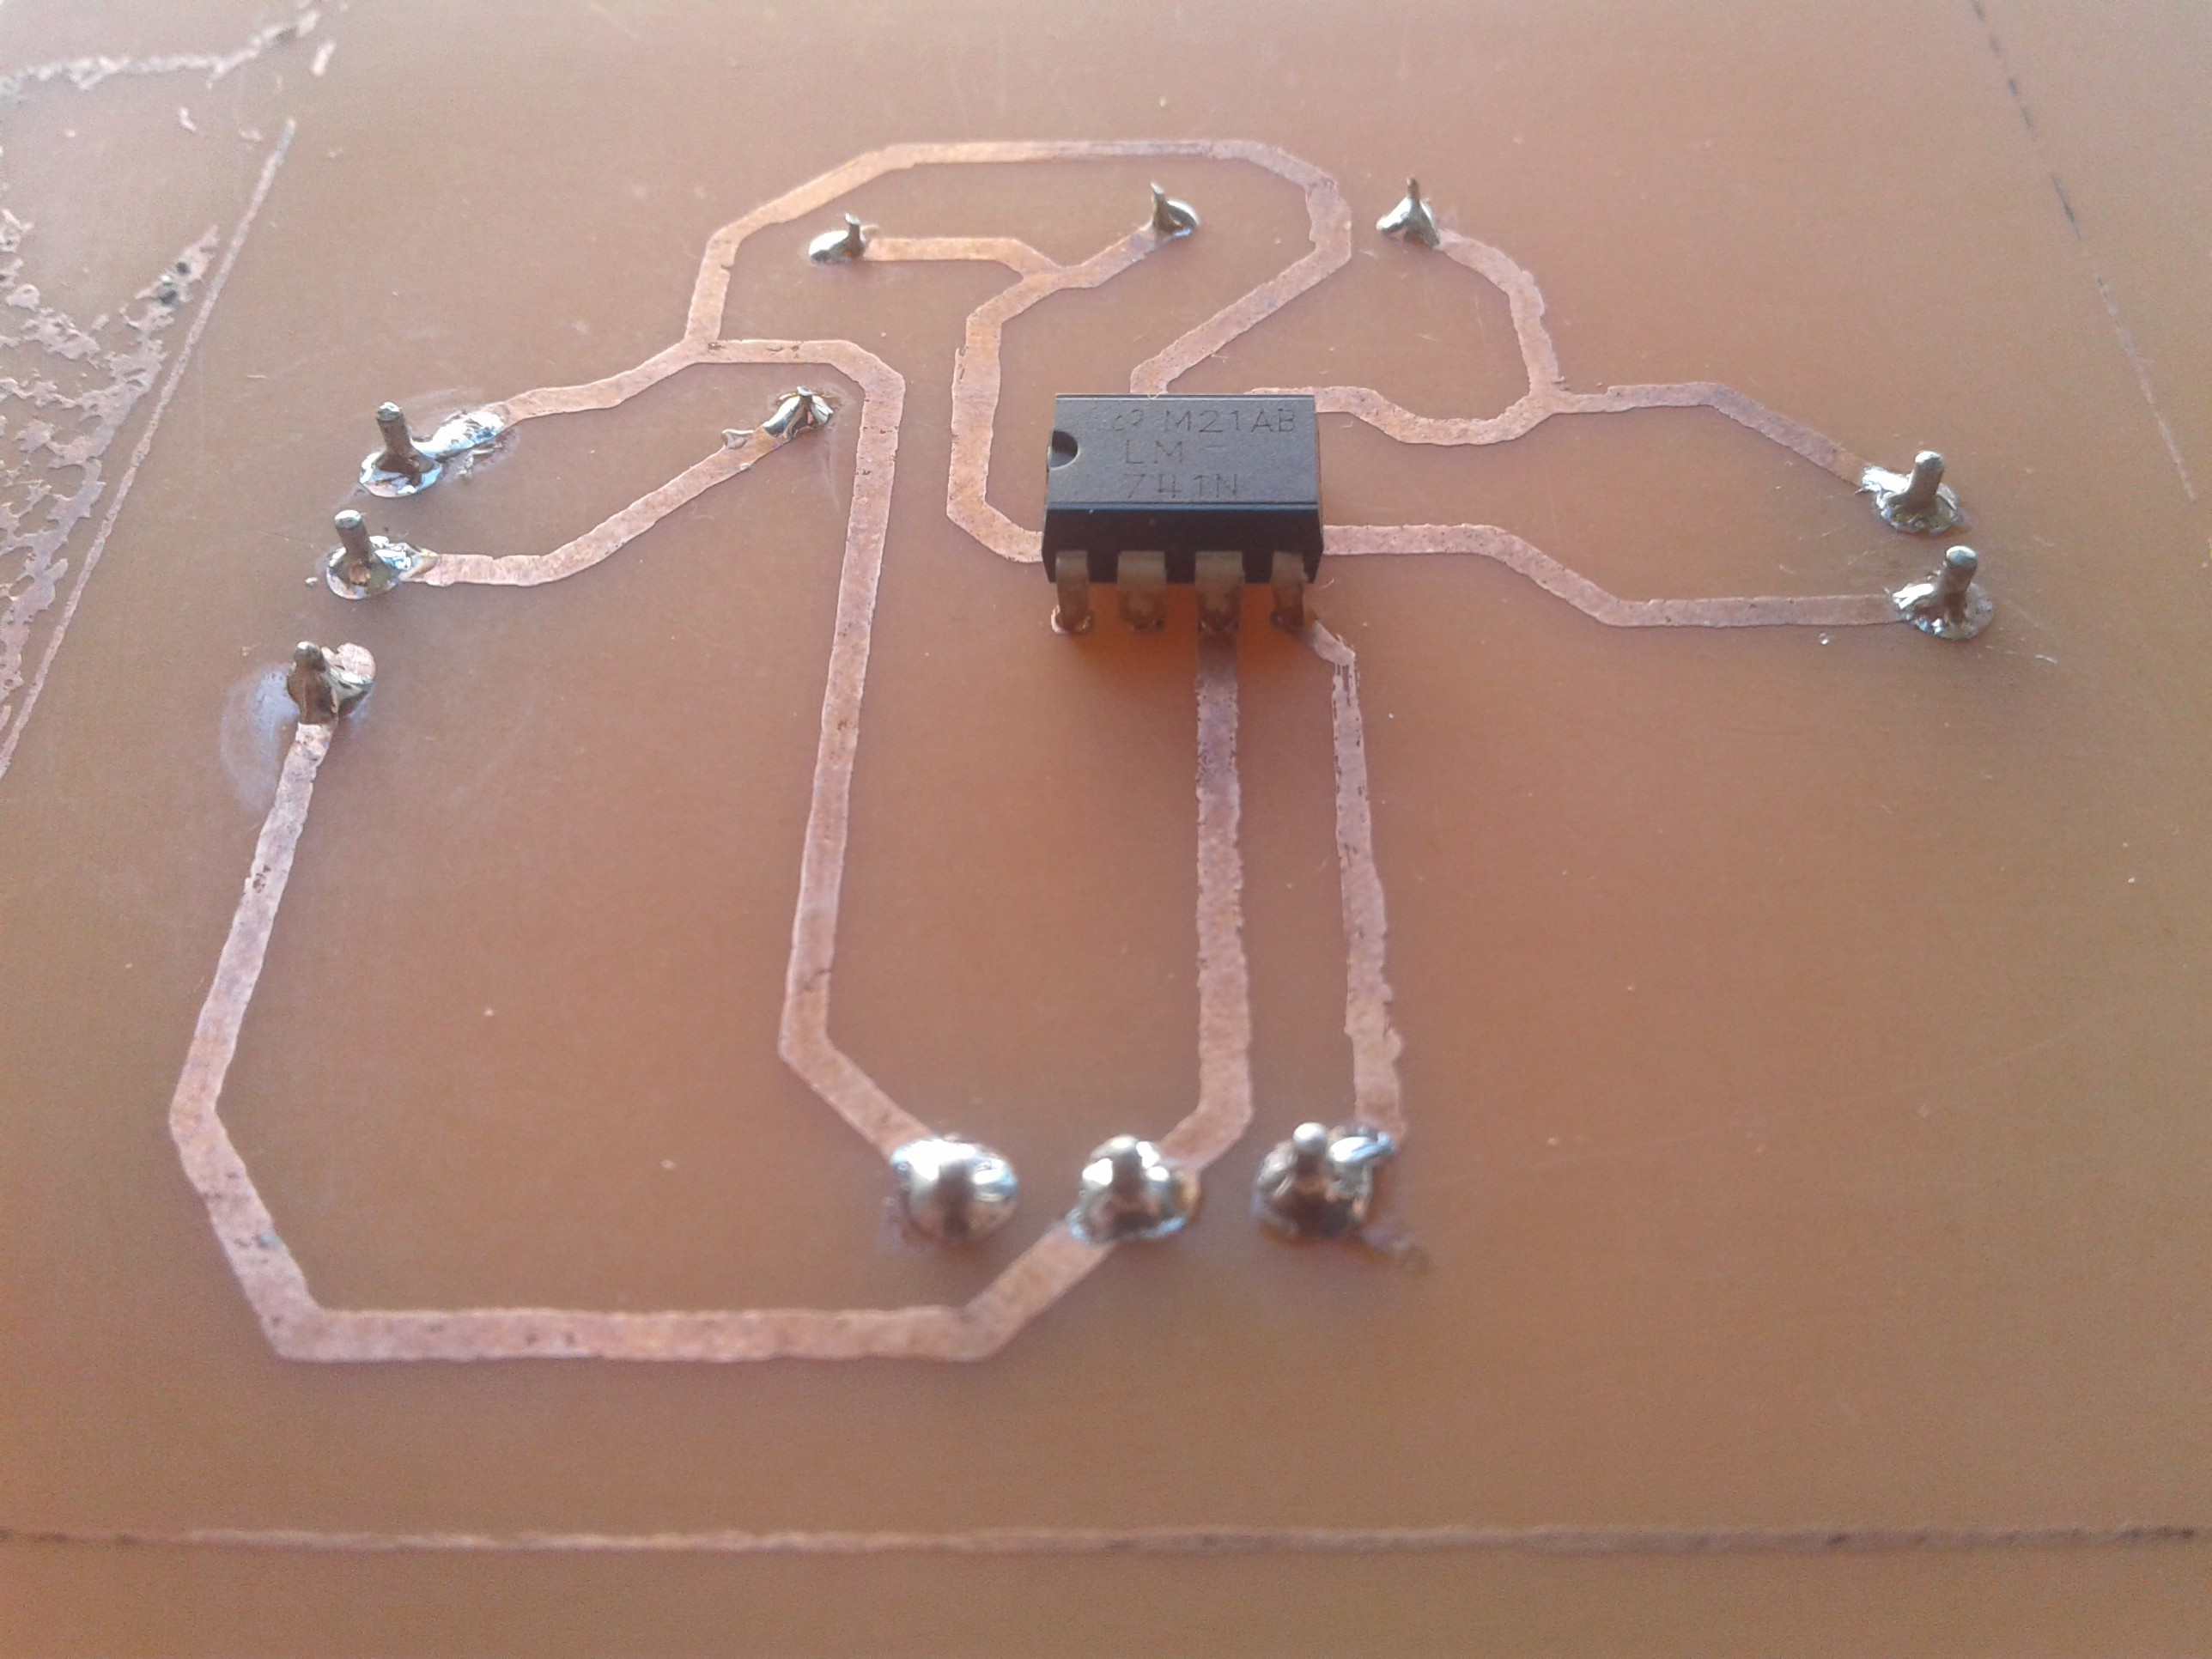
\includegraphics[width=5cm]{f2.jpg} }}%
                \caption{Fotos da placa}%
                \label{fig:example}%
            \end{figure}
        
                
                
                
\end{document}